\chapter{Implementation}
\label{4-practical}

\section{Functionality} 

PyWPS allows to publish and use geoprocessing services on a server. Every process that is to be implemented by PyWPS must be constructed as a Python class, contain a list of inputs nad outputs and a handler method with two parameters - request and response. \cite{pywpsprocess} Details on the procedure of creating new processes can be found in PyWPS documentation.

To send a request to PyWPS, an instance of PyWPS must be running. If it is, the request is handled and a response is generated and returned to the client. The response has a form of an XML file and includes different elemenents depending on the type of the request.

When an Execute request is called, a new, temporary folder is created in location specified in configuration file and input data is moved here. While the process is being executed, temporary files may be generated in this folder. For every process, it must be specified what the final output is. Once the execution is finished, the output is copied to a location that is accessible via the web. The temporary folder, containing input and output data and all the intermediate data that arose during the execution, is then deleted.

\subsection{Output Data Management}

\subsubsection{Current Options} 

The simplest option of delivering output data is to embed it in the XML response document. Either as plain text, GML or, in case of an image, base64 scheme. This is typically used when the output is relatively small. It is also the default option.

\begin{figure}[H] \centering
      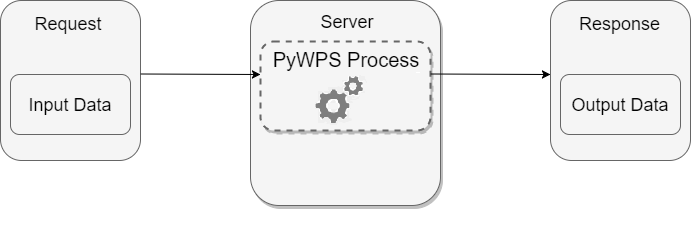
\includegraphics[width=350pt]{./pictures/optionone.png}
      \caption[Delivering data directly]{Delivering data directly}
      \label{fig:optionone}
  \end{figure}

If, on the contrary, the output data is large and complex, there is another option. The client is only given a reference, a URL link, from which the data can be downloaded. PyWPS saves the file in a folder specified in configuration passed by the service (or in a default location). The URL is embedded in the XML response. \cite{pywpsurl}

\begin{figure}[H] \centering
      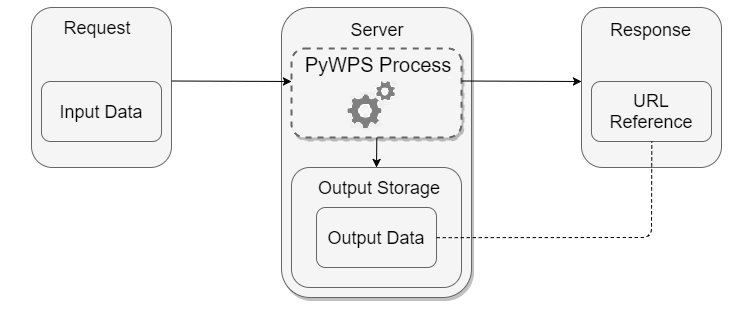
\includegraphics[width=370pt]{./pictures/optiontwo.png}
      \caption[Delivering data via URL reference]{Delivering data via URL reference}
      \label{fig:optiontwo}
  \end{figure}

It is up to the consumer of the process to decide which option to choose. For the latter option, the \texttt{"@asReference"} value must be set to \texttt{"True"}  in the request. \cite{asref} By default, it is set to \texttt{"False"}.


\subsubsection{Proposed Extension} 

The aim of this thesis was to develop another variant to add to the existing two that would store output data in a PostGIS database.

From the point of view of the consumer of a process, it is similar to the previous option. After the final output has been produced, connection to the database is established and the output data is copied there. When the XML response is delivered to the client, it contains a reference to the database with which the client can access the data. The reference is composed of the name of the database, schema and table. 

\begin{figure}[H] \centering
      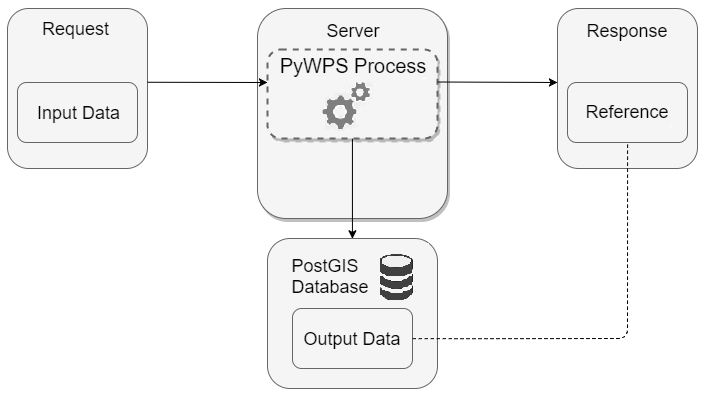
\includegraphics[width=350pt]{./pictures/newoption.png}
      \caption[Storing data in a database]{Storing data in a database}
      \label{fig:newoption}
  \end{figure}


%To use this functionality as a consumer of a process, it must be implemented in the process by its author. For details on implementation when creating a process, please refer to the User Manual.


\section{Development} 

\subsection{PgStorage class development} 

A new class, \texttt{PgStorage}, has been developed that implements database storage support. It is a derived class, inheriting from  \texttt{StorageAbstract} class that is a part of the standard PyWPS library. 

PgStorage is stored within \texttt{storage.py} in the .\textbackslash pywps\textbackslash inout folder. It consists of several methods that are described below. 

\subsubsection{\textunderscore \textunderscore init\textunderscore \textunderscore } 
A constructor, i.e. it gets called automatically when an instance of the \texttt{PgStorage} class is created. 

In this method, the \texttt{get\textunderscore config\textunderscore value}  function is used that is defined within the PyWPS API. It accesses the configuration file and retrieves required elements. What elements are retrieved is specified by the function's two parameters, section and option. 

First, the correct section (\texttt{db}) is specified and saved to a variable. Then, the name of the database is extracted from the configuration file and saved to a variable. 

Another variable is defined that serves as a connection string for connecting to a database. Requisite elements (user name, password and host server) are retrieved from the configuration file. Finally, an instance of the \texttt{\textunderscore create\textunderscore schema} method is created and saved to a variable.


\subsubsection{\textunderscore create\textunderscore schema} 
First defines a variable \texttt{schema\textunderscore name} as a random string of specified length that consists of letters and digits. This is done using Python libraries "random" and "string".  
 
%In the future, schema_name should be created in another way so it is related to the process

Next, \texttt{psycopg2} library is used to connect to the database, specified by the target variable. A try-except clause is used to raise an exception if the connection could not be established. 

Then, when a cursor has been created, an SQL query is executed that generates a new schema if it doesn't exist already. Name of the schema is equal to the \texttt{schema\textunderscore name} variable. This, too, uses a try-except clause.

After the SQL query is performed, changes in the database are commited so they persist after connection is aborted, cursor and connection are closed and the \texttt{schema\textunderscore name} variable is returned.

\subsubsection{\textunderscore store\textunderscore output} 
As its name suggests, it handles writing output data to the database. It benefits from an extensive use of the OGR library. It has two input parameters, the name of the file that is to be stored in a database, and a process identifier. 

Thanks to OGR, the process is fairly simple and straight-forward. The output file is opened using the file name input parameter and connection to the database is established. Then, data is copied from the output file to the database using the OGR CopyLayer function. 

Each of the three above mentioned operations is followed by a simple condition that checks if the variable storing output of the operation is not None. If it is, it raises an exception with a corresponding message.

This method returns the identifier.


\subsubsection{store} 

The store method is defined in the \texttt{StorageAbstract} parent class. Just as in the parent class, it has output as an input argument.

It initializies the \texttt{\textunderscore  store\textunderscore output} method and passes it name and identifier of the output file. 

Then, a string is created that specifies the location of the data and saved as a variable. It consists of a name of the database, schema and identifier. This string is then given to the client as an output in the XML response of the process.

There are three parameters returned by the method - the corresponding value of a DB variable defined within the \texttt{STORE\textunderscore TYPE} class, name of the output file and the variable describing the location of the data. These must be returned as they are required by the \texttt{get\textunderscore url} method (defined within the \texttt{ComplexOutput} class). 


\subsection{PyWPS source code changes} 

All changes that have been done within the PyWPS source code can be examined in a \texttt{diff} folder that is appended to this thesis. It contains a file for each of the three classes mentioned below that documents every alteration of the original code.

\subsubsection{Process.py class} 

The \texttt{Process} class is a part of the PyWPS source code. All processes inherit from this class. 

A snippet of code must be added at a specific location in one of the methods of the \texttt{Process} class, \texttt{\textunderscore run\textunderscore process}. It needs to be placed immediately after response is created.

It consists of a \texttt{hasattr} condition and a method call. The \texttt{hasattr} function is one of the functions built into the Python interpreter. It has two input parameters, name of an object and string. If the string is one of the object's attributes, it evaluates the condition as \texttt{"True"}. \cite{hasattr} In this case, the object is \texttt{self} and the string is \texttt{writer}. 

If the condition is met (i.e. the object - a process - does have an attribute called \texttt{writer}) the second line is executed and the \texttt{store} method is called.

\subsubsection{Outputs.py class}

Since there is another option being added of storing output data that returns a reference to the client, the \texttt{\textunderscore execute\textunderscore xml\textunderscore reference} method had to be adjusted.

Whether the output data is stored as a file or in a database depends on value of the \texttt{store\textunderscore type} option in configuration file. Therefore, the code block that has been added here first retrieves the value using \texttt{get\textunderscore config\textunderscore value}. If it is equal to \texttt{"db"}, \texttt{PgStorage} is chosen to handle output data. In any other case (the value is different or the option is missing), \texttt{FileStorage} is used.

\subsubsection{Storage.py class}

Here, the \texttt{PgStorage} class has been added that implements the database storage functionality. For more details on this class, please refer to the section 4.2.1.

Also, second option has been added to the class \texttt{STORE\_TYPE}. So, apart from a \texttt{PATH} variable that implies storing output data as a file, there is also a \texttt{DB} variable that is used when saving data in a database.

\subsection{Test} 

A script has been developed to test whether the process of storing outputs in a database functions correctly.

For the purpose of this test, three simple processes have been written. One of them only returns a string, other two, (\texttt{process\textunderscore one\textunderscore output} and \texttt{process\textunderscore two\textunderscore outputs}), produce one and two complex outputs, respectively. 

Both \texttt{process\textunderscore one\textunderscore output} and \texttt{process\textunderscore two\textunderscore outputs} generate buffers around input features, the latter also calculates centroids thereof. They are based on sample processes available for the PyWPS demo service. There is also a GML file provided with the demo service that was used as an input file for this test.  

To sucessfully run the test, instance of PyWPS must be running. When run, the test executes each of the processes and analyzes the corresponding XML response using the ElementTree XML parser. For every process, it returns an identifier of the process extracted from the XML document. 

For the two processes that yield complex outputs the test establishes connection to the database and counts features in the corresponding table. Then it compares this value to the number of features in the input file. If these two values differ, it raises an exception.

Similarly, it checks whether the geometry type of the layer in database is equal to a predefined value (point for centroids, polygon for buffer). If not, it raises an exception with a corresponding warning. 

When no exception is raised, it indicates that all processes have been run and all complex outputs have been stored in a database.

The OGR library is used for creating database connection, counting features and getting geometry type. Database login credentials are retrieved from a configuration file using \texttt{get\textunderscore config\textunderscore value}. To ensure correct configuration file is read, another PyWPS built-in function, \texttt{load\textunderscore configuration}, is used.







